\NewDocumentCommand{\drawunit}{mm}
{
    \lPoint{O}{#1}
    \lShift{A}{O}{\fpeval{#2+90}:0.125}
    \lShift{B'}{A}{\fpeval{#2+180}:0.3}
    \lShift{C'}{A}{\fpeval{#2+0}  :0.3}
    \lShift{B}{B'}{\fpeval{#2-90}:0.25}
    \lShift{C}{C'}{\fpeval{#2-90}:0.25}
    \draw[rotate=#2,very thin,fill=blue!20!white] (A) rectangle (B);
    \draw[rotate=#2,very thin,fill=red!20!white ] (A) rectangle (C);
    \lRatio{Btext}{A}{B}{0.5}
    \lRatio{Ctext}{A}{C}{0.5}
    \node[rotate=#2] at (Btext) {\footnotesize S};
    \node[rotate=#2] at (Ctext) {\footnotesize N};
}

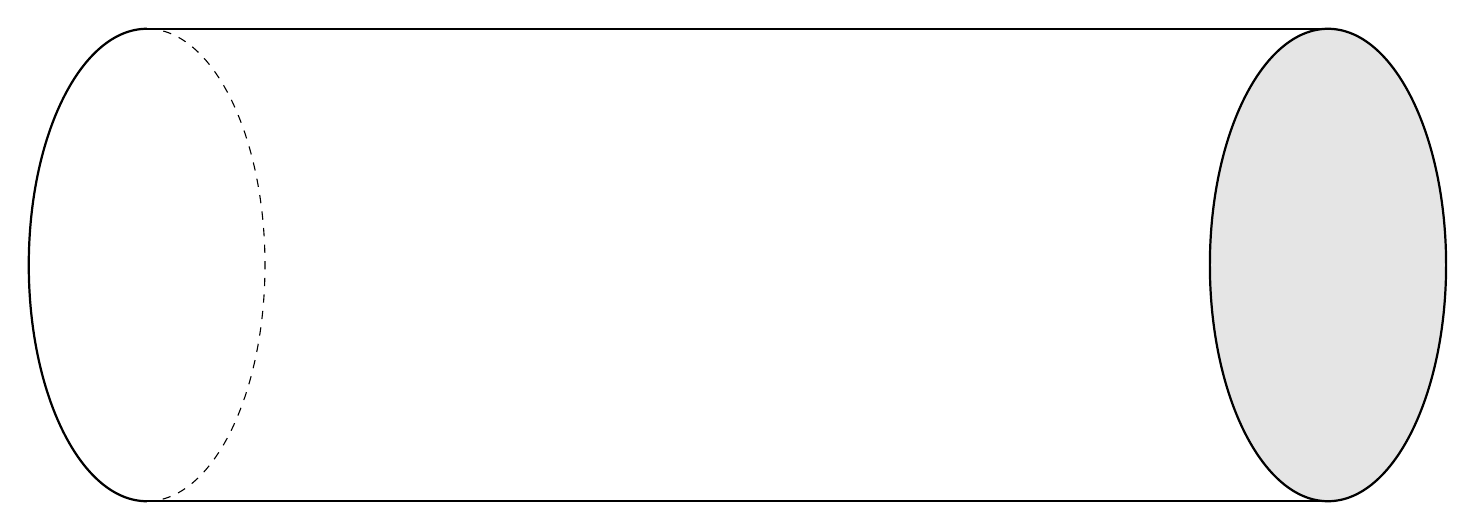
\begin{tikzpicture}[scale=1.5]
    \foreach \i in {-5,-4,...,5}
    {
        \foreach \j in {-1.2,-0.4,0.4,1.2}
        {
            \drawunit{\i,\j}{0}
        }
    }
    \draw[thick](+5,0) ellipse (1 and 2);
    \draw[thick](-5,2) arc (90:270:1 and 2);
    \draw[dashed](-5,2) arc (90:-90:1 and 2);
    \draw[thick] (-5,+2)--(+5,+2);
    \draw[thick] (-5,-2)--(+5,-2);
    \fill[fill=black,fill opacity=0.1](+5,0) ellipse (1 and 2);
\end{tikzpicture}
